\documentclass[a4paper,12pt]{article}
\usepackage[a4paper,top=1.3cm,bottom=2cm,left=1.5cm,right=1.5cm,marginparwidth=0.75cm]{geometry}
\usepackage{cmap}
\usepackage{mathtext}
\usepackage[T2A]{fontenc}
\usepackage[utf8]{inputenc}
\usepackage[english,russian]{babel}
\usepackage{siunitx}
\usepackage{enumitem}
\usepackage{placeins}

\usepackage{graphicx}
\usepackage{amsmath}

\usepackage{wrapfig}
\usepackage{tabularx}
\usepackage{multirow}

\usepackage{hyperref}
\usepackage[rgb]{xcolor}
\hypersetup{colorlinks=true,urlcolor=blue}
\usepackage{siunitx}
\usepackage{amsmath,amsfonts,amssymb,amsthm,mathtools}
\usepackage{mathtools}
\usepackage{icomma}
\mathtoolsset{showonlyrefs=false}
\usepackage{euscript}
\usepackage{mathrsfs}
\DeclareMathOperator{\sgn}{\mathop{sgn}}
\newcommand*{\hm}[1]{#1\nobreak\discretionary{}
{\hbox{$\mathsurround=0pt #1$}}{}}

%%% Заголовок
\newcommand\labname{Спектрометрия $\alpha$-излучения с помощью полупроводникового детектора}
\newcommand\labnumber{5.2}


\author{Макаров Лев Евгеньевич}
\title{Лабораторная работа №\labnumber

\labname
}

\date{\today}

\begin{document}

\begin{titlepage}
	\begin{center}
		{\large МОСКОВСКИЙ ФИЗИКО-ТЕХНИЧЕСКИЙ ИНСТИТУТ (НАЦИОНАЛЬНЫЙ ИССЛЕДОВАТЕЛЬСКИЙ УНИВЕРСИТЕТ)}
	\end{center}
	\begin{center}
		{\large Физтех-школа фотоники, электроники и молекулярной физики}
	\end{center}
	
	
	\vspace{4.5cm}
	{\huge
		\begin{center}
			{\bf Отчёт о выполнении лабораторной работы \labnumber}\\
			\labname
		\end{center}
	}
	\vspace{2cm}
	\begin{flushright}
		{\LARGE Автор:\\ Макаров Лев Евгеньевич \\
			\vspace{0.2cm}
			Б04-306}
	\end{flushright}
	\vspace{8cm}
	\begin{center}
		Долгопрудный 2025
	\end{center}
\end{titlepage}

\section{Введение}

\textbf{Цель работы:} 
\begin{enumerate}
	\item С помощью кремниевого поверхностно-барьерного детектора измерить спектры $\alpha$-частиц, испускаемых различными радиоактивными ядрами — $\prescript{226}{88}{\text{Ra}}, \prescript{241}{95}{\text{Am}} + \prescript{230}{90}{\text{Th}}, \prescript{239}{94}{\text{Pu}}$ и $\text{U}_\text{пр}$.
    \item По их величине определить энергию $\alpha$-частиц.
    \item Проверить выполнение закона Гейгера-Неттола.
\end{enumerate}


\section{Теоретические сведения}

\subsection*{Свойства $\alpha$-распада}

Энергию вылетающих из ядра $\alpha$-частиц легко подсчитать на основе законов сохранения.

\begin{equation}\label{eq:1}
    M_2 c^2 =M_1 c^2 + m_\alpha c^2 + T_1 + T_\alpha
\end{equation}
\begin{equation}\label{eq:2}
    \mathbf{p_1} + \mathbf{p_\alpha} = 0
\end{equation}

Ясно, что вылет $\alpha$-частицы из ядра возможен лишь в том случае, если разность энергий покоя родительского и дочернего ядра будет больше энергии покоя $\alpha$-частицы. В силу того, что реально $\alpha$-распад испытывают лишь тяжелые ядра с $A > 200$, энергия отдачи ядра очень мала и фактически кинетическая энергия $\alpha$-частицы равна разности энергий покоя исходного и конечного ядер. Именно поэтому вылетающие $\alpha$-частицы имеют строго определенную энергию.


Однако экспериментально обнаружено, что энергетический спектр $\alpha$-частиц многих $\alpha$-активных ядер состоит из нескольких линий, одна из которых является преобладающей. В качестве примера на рис. \ref{pic:spectre} показан $\alpha$-спектр ($\prescript{212}{83}{\text{Bi}}$).


Дискретность линий и их относительная интенсивность объяснимы, поскольку, во-первых, $\alpha$-частицы могут испускаться ядром, находящимся в возбужденном состоянии (так называемые длиннопробежные $\alpha$-частицы), а во-вторых, может происходить $\alpha$-распад из основного состояния родительского ядра на возбужденные состояния дочернего ядра (короткопробежные $\alpha$-частицы). На рис. \ref{pic:Pu_Po} приведены два примера таких переходов — распад $\prescript{238}{}{\text{Pu}}$ и $\prescript{212}{}{\text{Po}}$.

\FloatBarrier
\begin{figure}[h]
    \begin{center}
        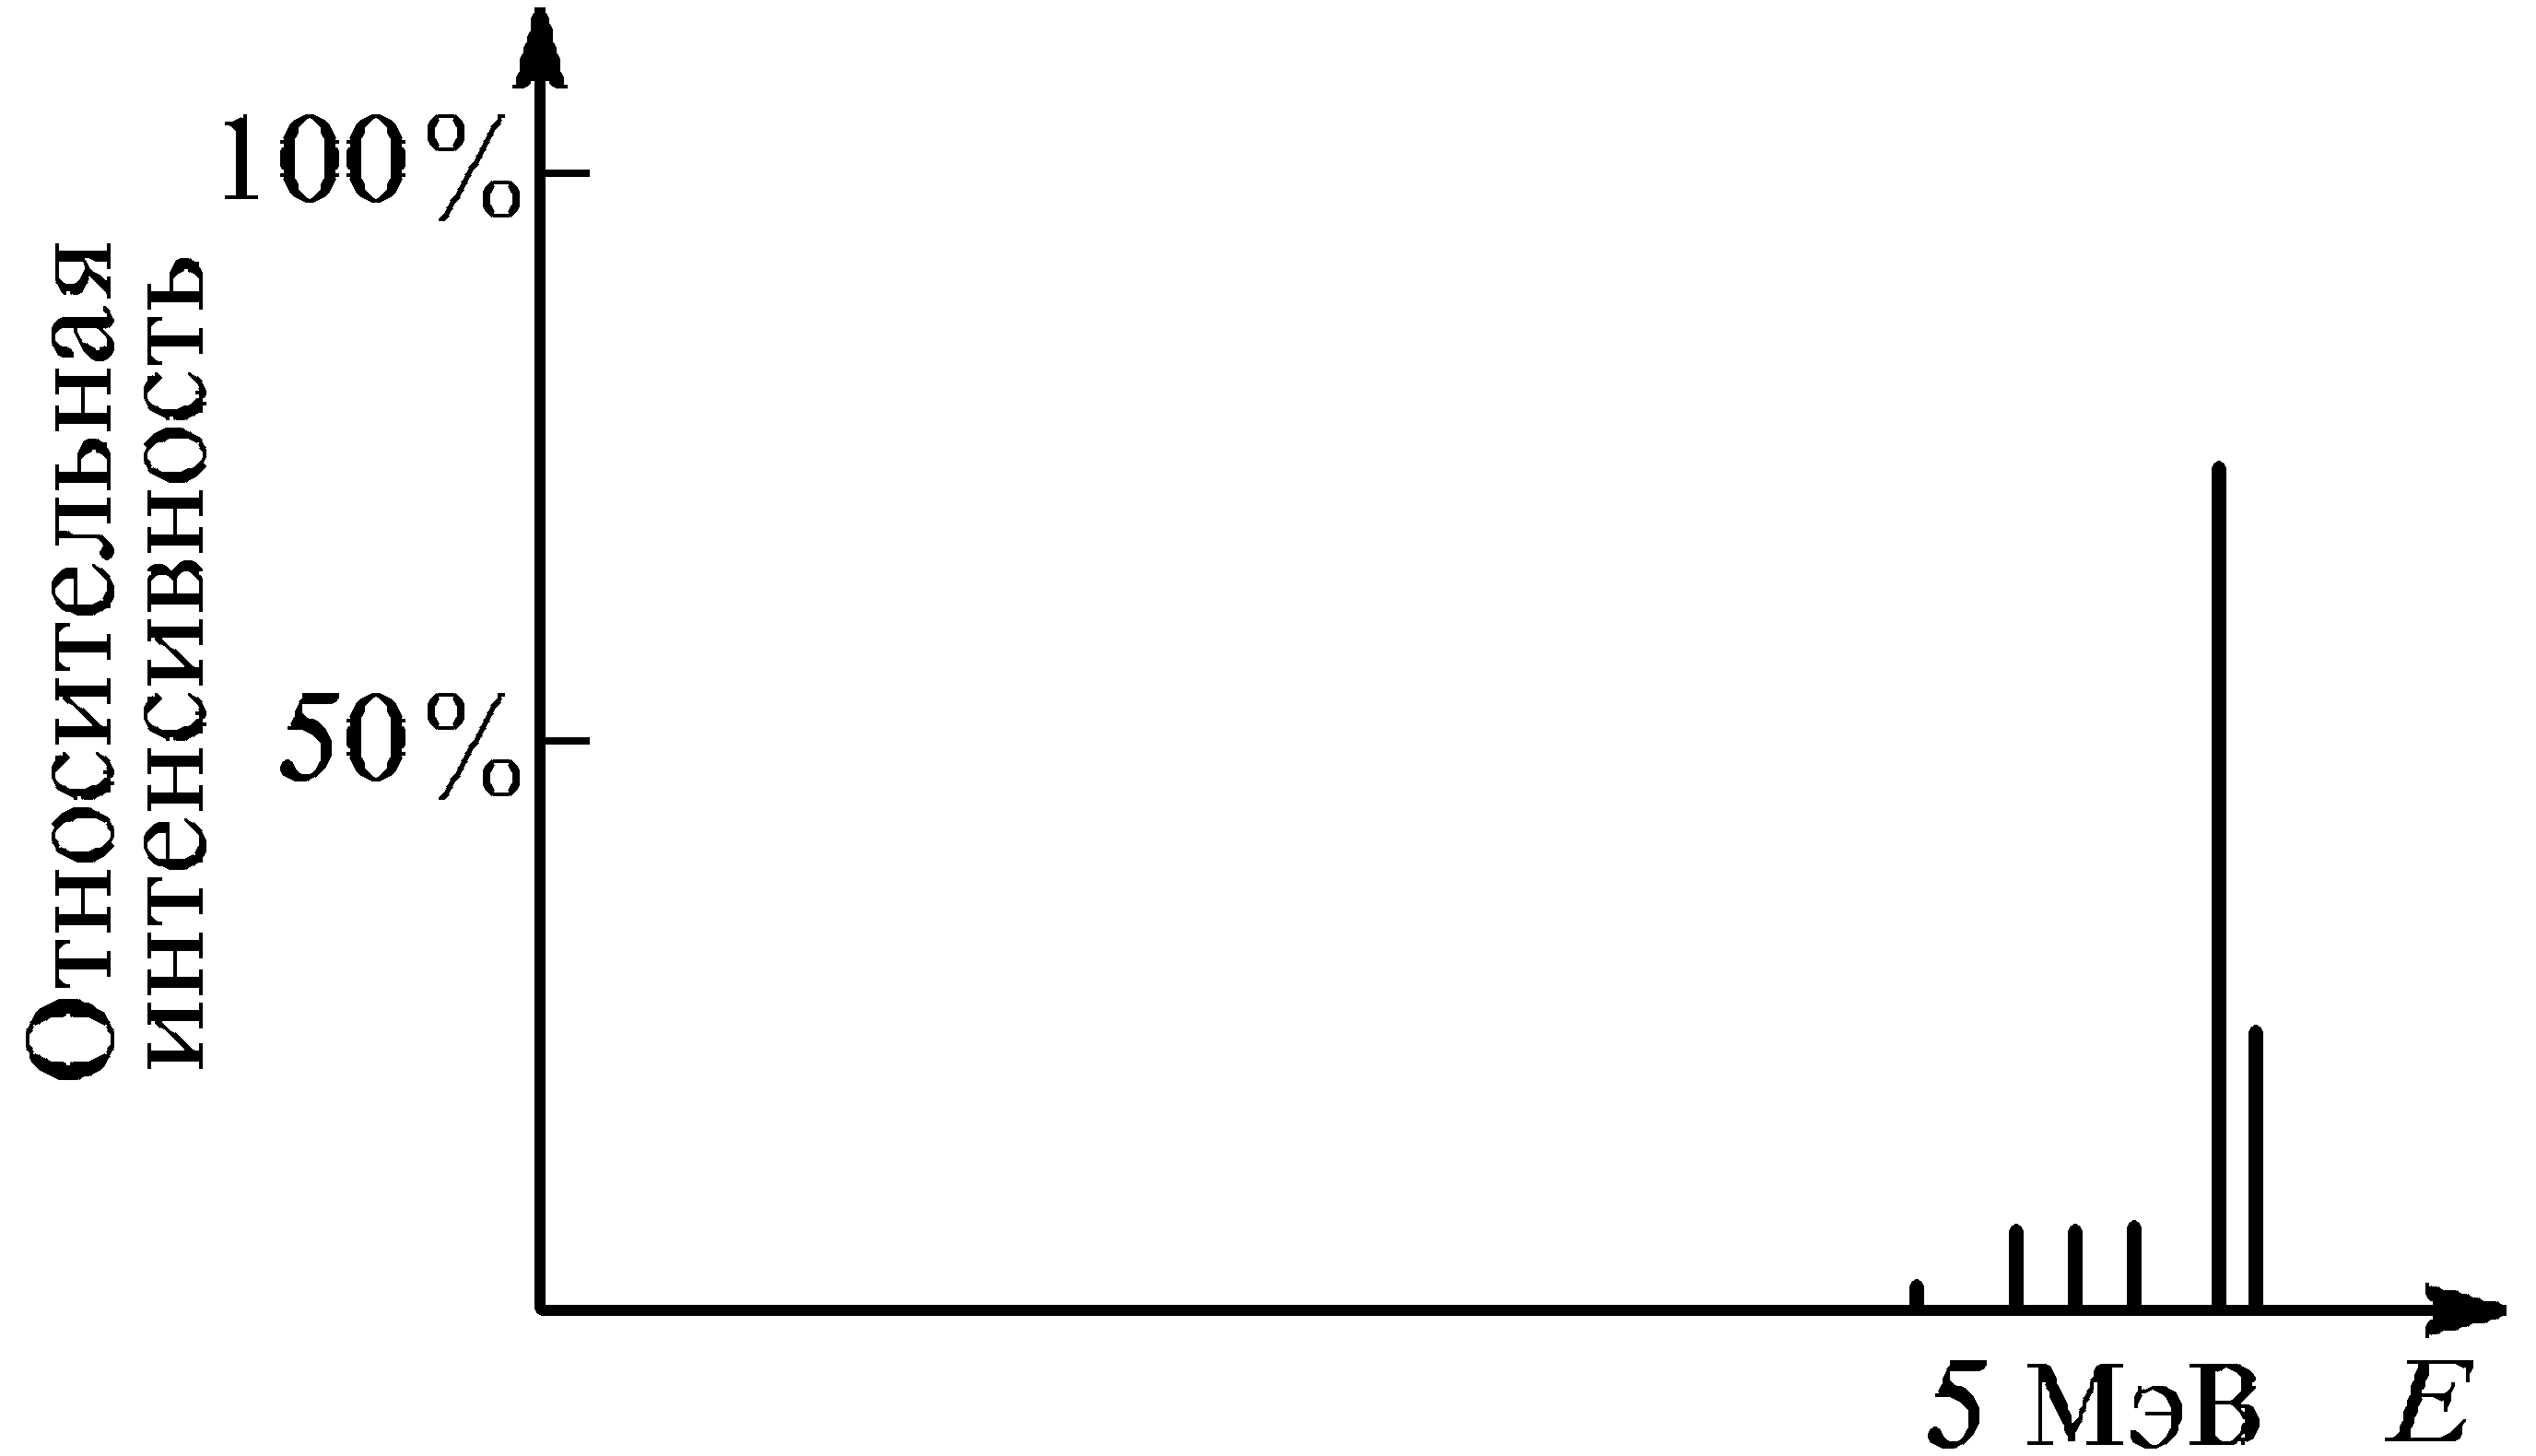
\includegraphics[width = 0.7\textwidth]{pics/spectre.png}
        \caption{Энергетический спектр $\alpha$-частиц, вылетающих при распаде $\prescript{212}{83}{\text{Bi}}$}
    \label{pic:spectre}
    \end{center}
\end{figure}
\FloatBarrier


В первом случае ($\prescript{238}{}{\text{Pu}}$) $\alpha$-частицы максимальной энергии соответствуют переходам из основного состояния $\prescript{238}{}{\text{Pu}}$ в основное состояние дочернего ядра. Кроме того, $\alpha$-распад может идти на возбужденные состояния дочернего ядра $\prescript{234}{}{\text{U}}$ с последующими $\gamma$-переходами в основное состояние. Распад $\prescript{212}{}{\text{Po}}$ — пример возможности испускания $\alpha$-частиц из возбужденного состояния. Такая ситуация возникает из-за того, что $\prescript{212}{}{\text{Po}}$ образуется в результате $\beta$-распада $\prescript{212}{}{\text{Bi}}$. Находясь в возбужденном состоянии, ядро $\prescript{212}{}{\text{Po}}$ может либо испустить $\alpha$-частицу, либо путем $\gamma$-излучения перейти в основное состояние. Так как период полураспада для $\alpha$-частиц примерно в 105 раз больше периода $\gamma$-распада, то интенсивность длиннопробежных $\alpha$-частиц очень мала.

\FloatBarrier
\begin{figure}[h]
    \begin{center}
        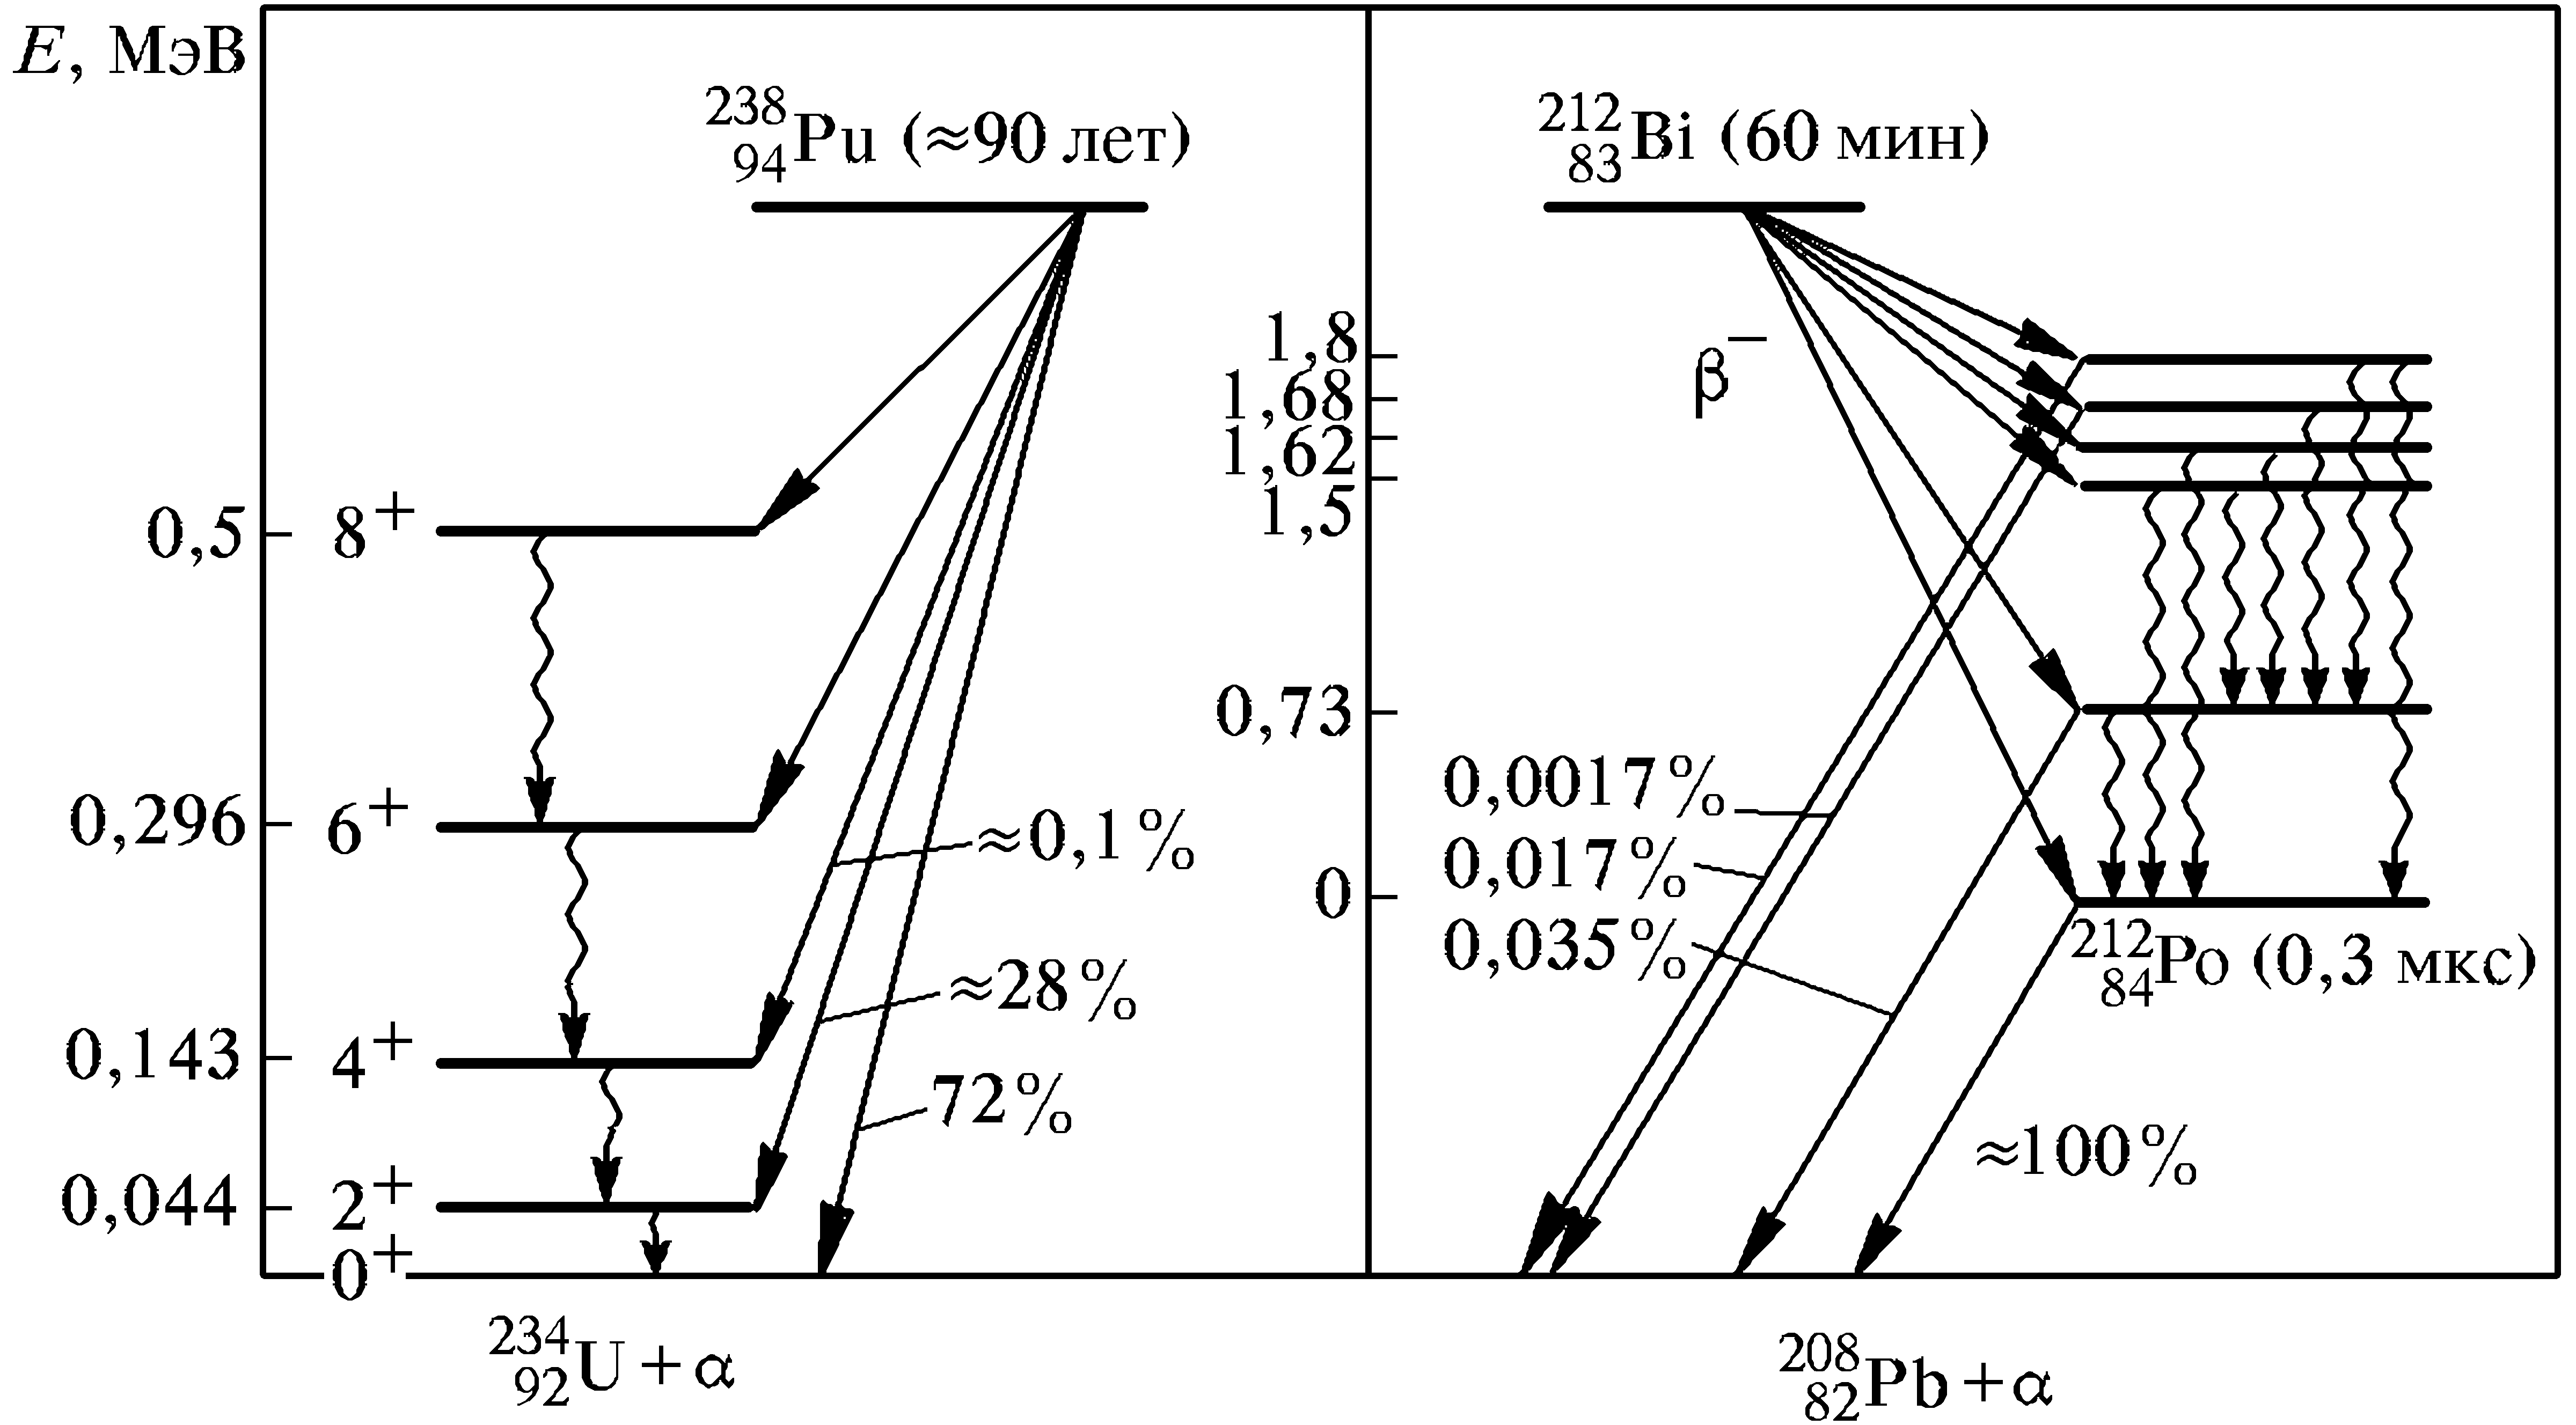
\includegraphics[width = 0.7\textwidth]{pics/PU_Po.png}
        \caption{Альфа-спектры распада ядер $\prescript{238}{}{\text{Pu}}$ и $\prescript{212}{}{\text{Po}}$}
    \label{pic:Pu_Po}
    \end{center}
\end{figure}
\FloatBarrier


Возбужденные состояния обладают разными спинами и четностью, а значит, разность моментов количества движения исходного и конечного ядра должна уноситься $\alpha$-частицей. Иными словами, $\alpha$-распад происходит с изменением углового момента ядра. Как показывают простые



оценки, если $\alpha$-частица имеет малый импульс $L$, то величина возникающего центробежного барьера составляет в тяжелых ядрах примерно $0.002L^2 A^2 = 0.002l(l + 1)$ часть от величины кулоновского барьера. Тем самым видно, что влияние центробежного барьера может быть существенным лишь для больших значений $l$. Тяжелые ядра, как правило, в основном состоянии деформированы (исключением являются магические ядра). Это означает, что низколежащими состояниями являются вращательные полосы, и именно на эти состояния обычно и происходит распад родительского ядра, приводящий к появлению группы короткопробежных $\alpha$-частиц. Как известно, энергия вращательных уровней определяется выражением


\begin{equation}\label{eq:3}
    E_\text{вр} = \frac{\hbar}{2I} l (l + 1)
\end{equation}


Тем самым измерение тонкой структуры энергетического спектра $\alpha$-частиц дает возможность определить момент инерции ядра $I$. Периоды полураспада $\alpha$-активных ядер очень сильно зависят от энергии вылетающих частиц. Экспериментально установленная зависимость (закон Гейгера–Нэттола) имеет вид:

\begin{equation}\label{eq:4}
    \lg T_{1/2} = \frac{a}{\sqrt{E_\alpha}} + b
\end{equation}


Коэффициенты a и b очень слабо зависят от заряда ядра $Z$.


\subsection*{Радиоактивные ряды}

Семейство $\prescript{238}{}{\text{U}}$, показанное на рис. \ref{pic:chain}, является нестабильной цепочкой превращений. Начинается с $\alpha$-активного изотопа урана $\prescript{238}{92}{\text{U}}$, который с периодом полураспада $4.5 \cdot 10^9$ лет превращается в $\prescript{234}{90}{\text{Th}}$ и т. д. Среди ядер этого семейства урана находится изотоп радия $\prescript{226}{88}{\text{Ra}}$, последовательность распадов которого изучается в данной работе. Очень скоро после приготовления моноизотопа $\prescript{226}{88}{\text{Ra}}$ ($T_{1/2} = 1617$ лет) в препарате накапливаются его дочерние продукты — $\prescript{222}{86}{\text{Rn}}$ ($T_{1/2} = 3.8$ дней), $\prescript{218}{84}{\text{Po}}$ ($T_{1/2} = 3$ мин) и $\prescript{214}{84}{\text{Po}}$ ($T_{1/2} = 10$ с), которые сами являются $\alpha$-активными. Поэтому при измерении $\alpha$-спектра радия-226 мы фактически наблюдаем $\alpha$-частицы, испускаемые всеми его дочерними продуктами.


\FloatBarrier
\begin{figure}[h]
    \begin{center}
        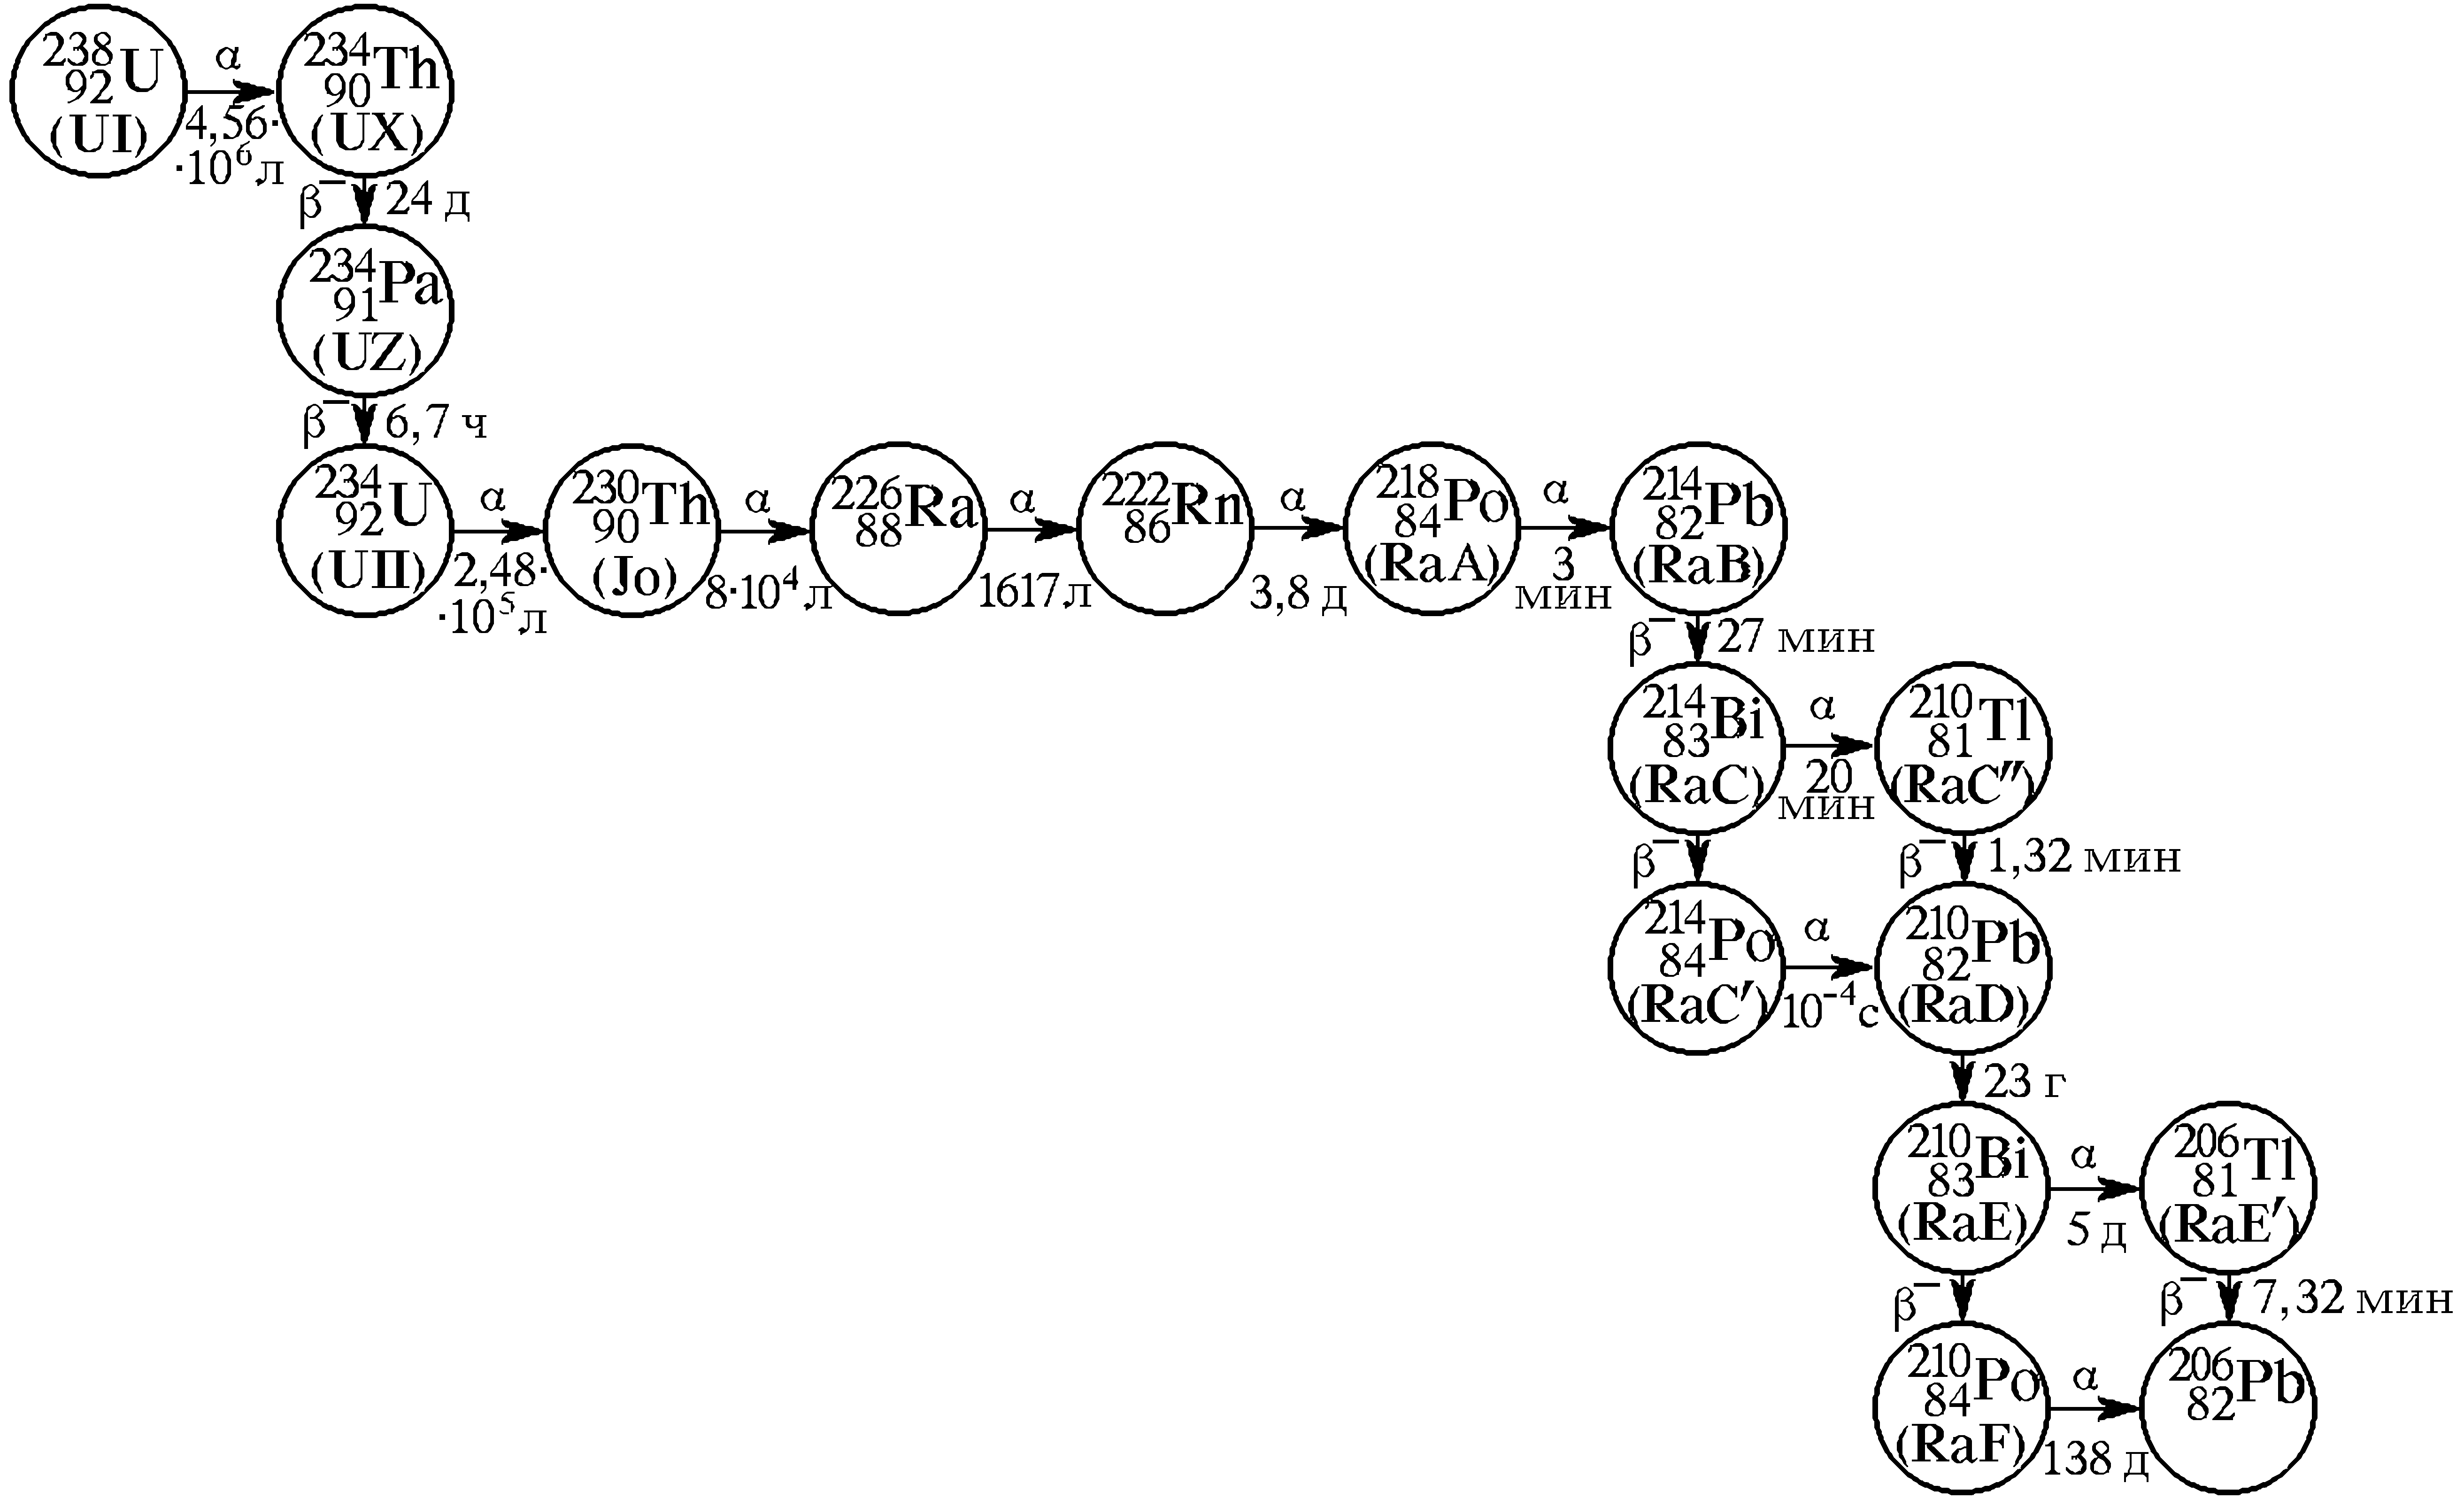
\includegraphics[width = 1\textwidth]{pics/chain.png}
        \caption{Последовательность радиоактивных превращений $\prescript{238}{}{\text{U}} \to \prescript{206}{}{\text{Pb}}$}
    \label{pic:chain}
    \end{center}
\end{figure}
\FloatBarrier


\section{Экспериментальная установка}

Основой установки является спектрометр $\alpha$-излучения. Конструктивно спектрометр выполнен в виде трех отдельных частей: измерительного модуля, персональной ЭВМ со встроенной платой амплитудноцифрового преобразователя (АЦП) и системы откачки СО вакуумной камеры ВК с блоком индикации БИ (см. рис. \ref{pic:ustan}).


В измерительном блоке смонтированы:
\begin{enumerate}[label=\arabic*)]
    \item вакуумная камера ВК, в которой расположен держатель образцов, поверхностно-барьерный полупроводниковый детектор и индикатор давления;
    \item малошумящий предварительный усилитель ПУ;
    \item спектрометрический усилитель СУ с органами управления;
    \item регулируемый блок низковольтного смещения БНС для питания детектора.
\end{enumerate}


Вакуумный насос создает в измерительной камере давление не более 10-2 Тор. Полупроводниковый детектор регистрирует $\alpha$-частицы с энергиями от 3.5 до 9 МэВ, его энергетическое разрешение составляет не более 30 кэВ при энергии $\alpha$-частицы 5 МэВ.


В поверхностно-барьерных полупроводниковых счетчиках преобразование энергии падающих частиц в электрические импульсы происходит в области так называемого (p–n)-перехода. Такой переход создается в виде тонкого слоя на границе между областями с p- и n-проводимостью. При прохождении частицы через обедненный слой вдоль ее трека создаются электронно-дырочные пары. Образовавшиеся носители разносятся электрическим полем (p–n)-перехода в разные стороны — и через кристалл проходит токовый импульс.

\FloatBarrier
\begin{figure}[h]
    \begin{center}
        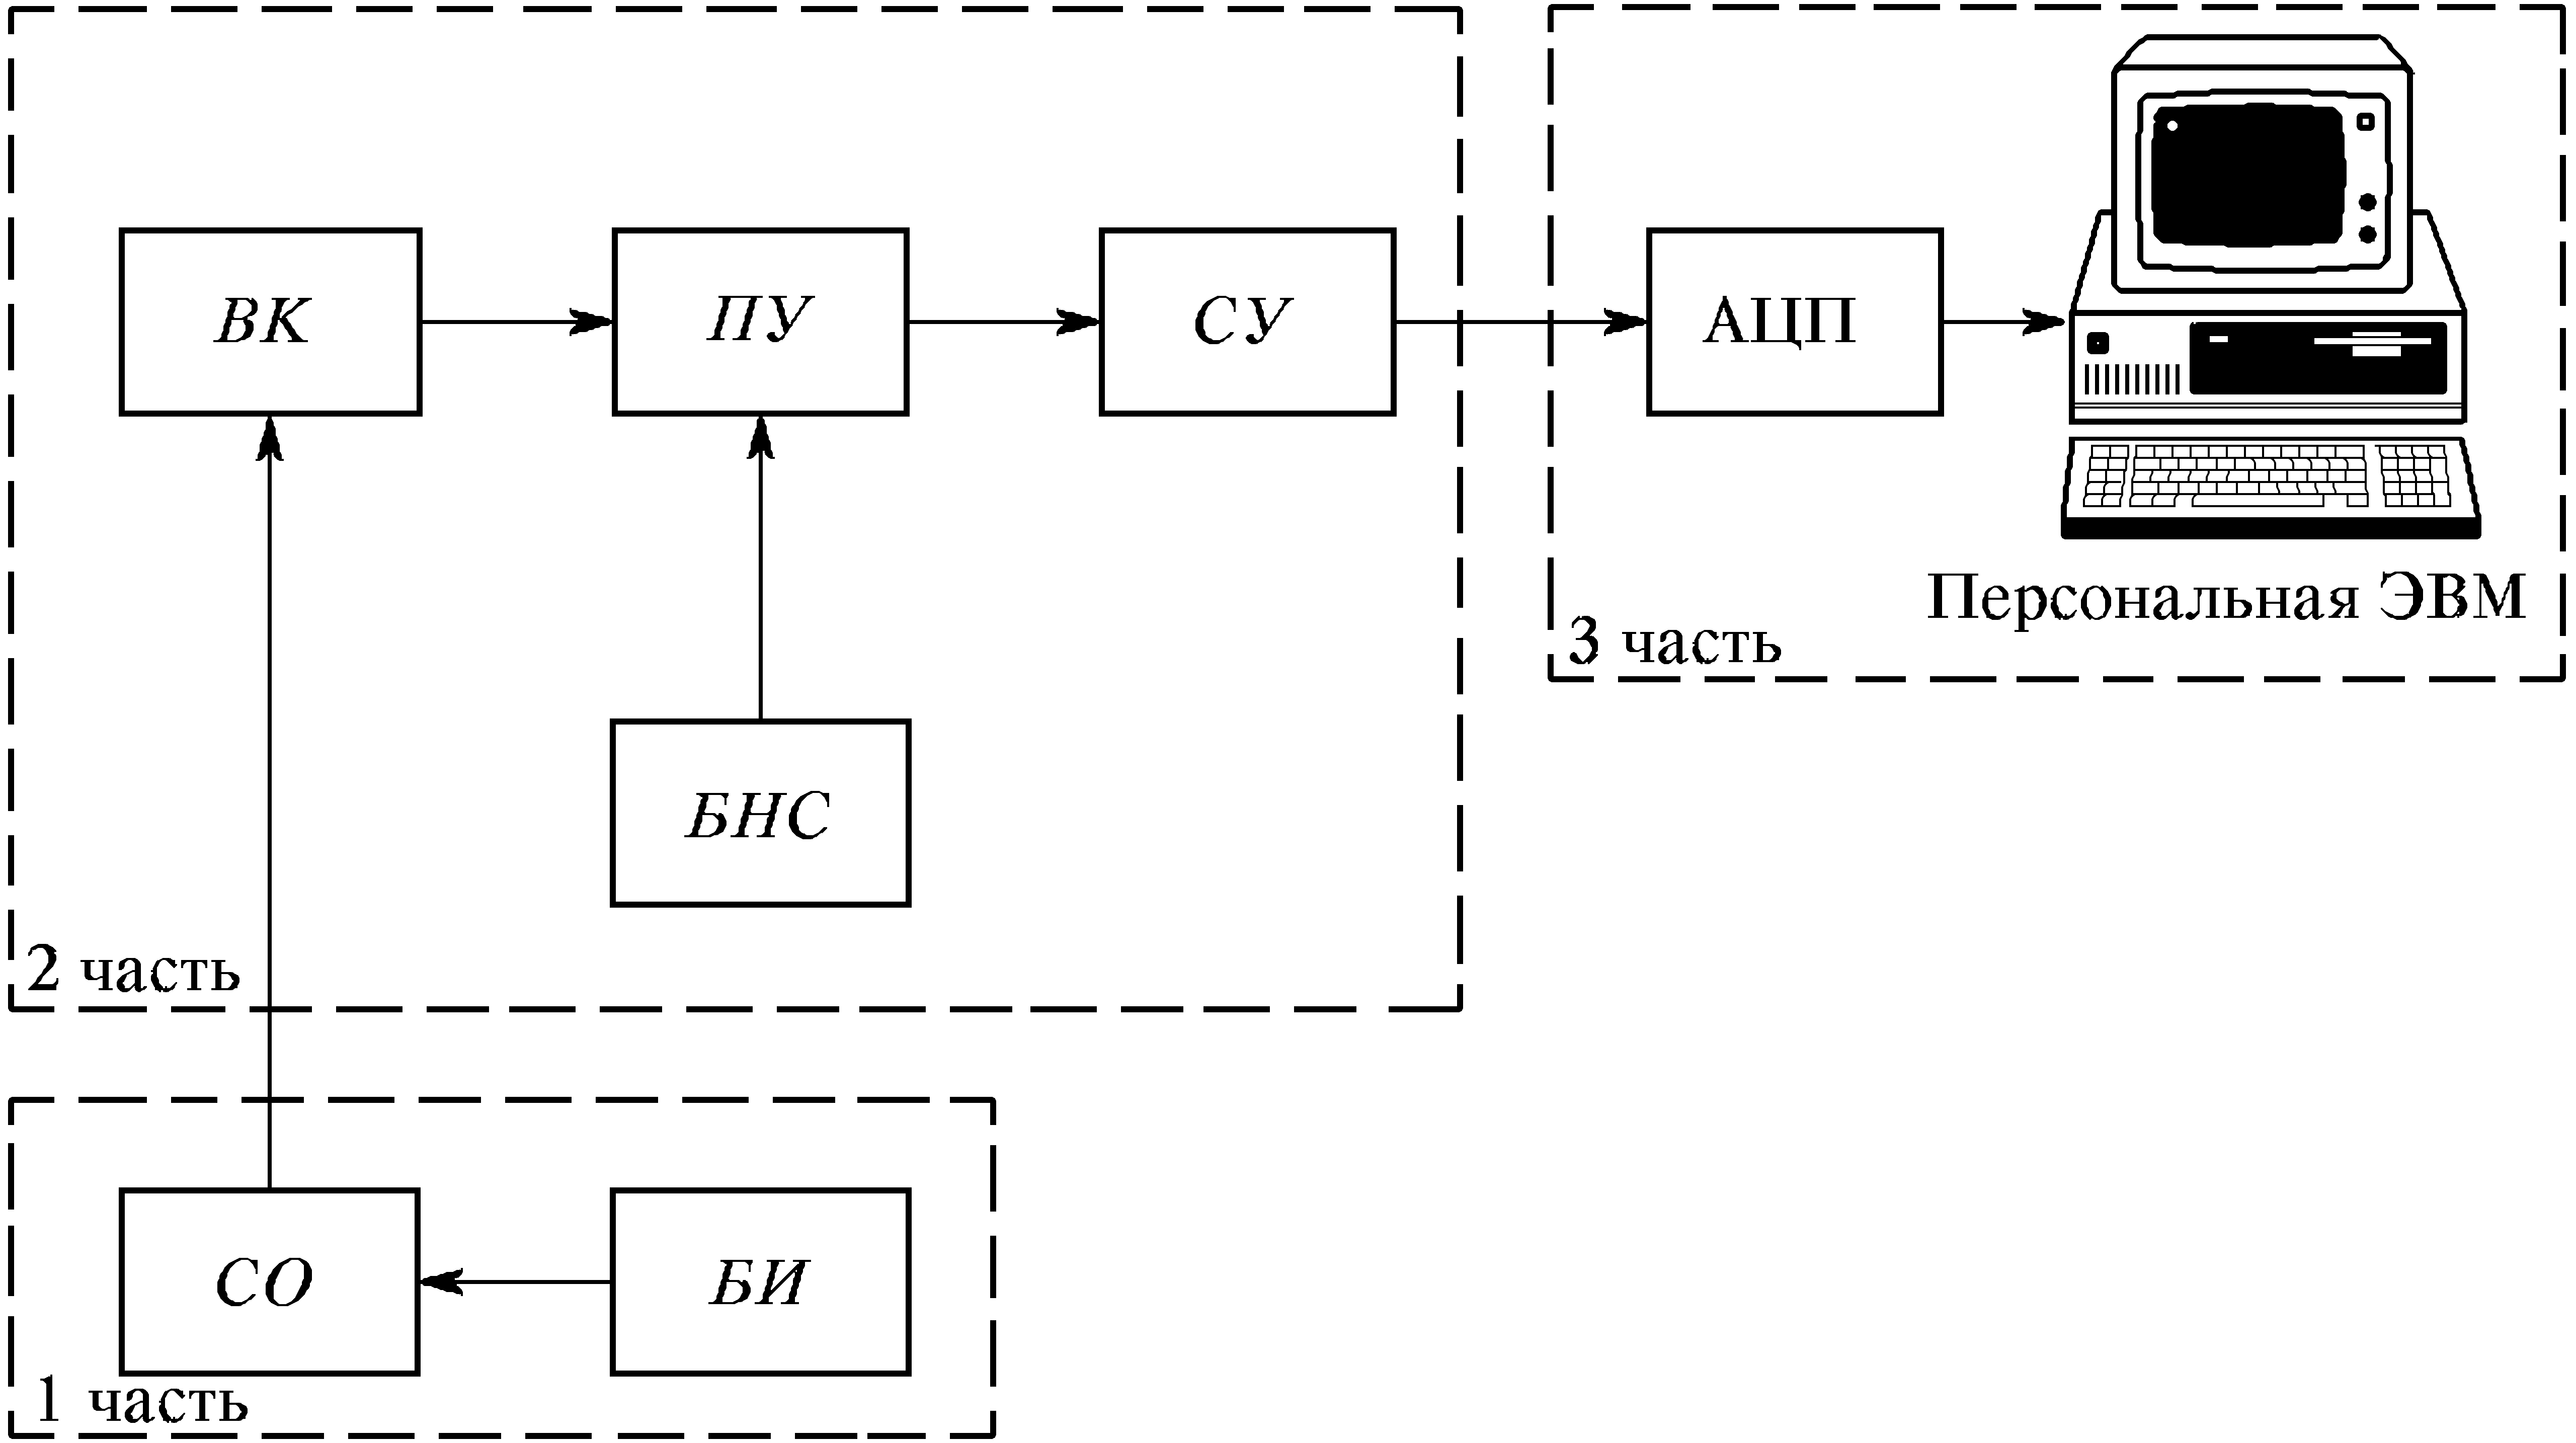
\includegraphics[width = 1\textwidth]{pics/ustan.png}
        \caption{Блок-схема спектрометра $\alpha$-излучения}
    \label{pic:ustan}
    \end{center}
\end{figure}
\FloatBarrier

При использовании детектора в спектрометрических целях особое значение приобретает его разрешающая способность, т. е. ширина кривой распределения импульсов по амплитудам при строго постоянной энергии регистрируемых частиц. Форма такой кривой распределения обычно бывает близка к кривой ошибок (гауссовой кривой)

\begin{equation}\label{eq:5}
    W (U) dU = \frac{1}{\sqrt{2 \pi} \sigma} e ^ { - (U - U_0)^2 / (2 \sigma^2) } dU
\end{equation}

десь $U_0$ — среднее значение амплитуды импульсов, $U$ — конкретное значение этой амплитуды, $W (U )dU$ — вероятность того, что при энергии частицы $E$ амплитуда измеренного импульса заключена между $U$ и $U + dU$, $\sigma$ — параметр, определяющий ширину распределения (среднеквадратичное отклонение).


Распределение \eqref{eq:5} имеет вид колокола с максимумом при $U = U0$.Разрешающую способность спектрометра определяют по величине $\delta$ — ширине кривой $W (U)$, измеренной на половине высоты. Энергетическим разрешением спектрометра обычно называют величину

\begin{equation}\label{eq:6}
    R = \frac{\delta}{U_0} \cdot 100 \%
\end{equation}

Нетрудно найти связь между $\delta$ и $\sigma$:


\begin{equation}\label{eq:7}
    \delta = 2 \sqrt{2 \ln 2} \sigma
\end{equation}


Одной из основных причин, вызывающих разброс импульсов по амплитуде, является статистическая флуктуация числа электрон-дырочных пар, создаваемых падающей частицей. Среднее число пар $N$ равно

\begin{equation}\label{eq:8}
    N = E / \mathcal{E}_\text{ср}
\end{equation}

где $E$ — энергия, теряемая частицей в детекторе, а $\mathcal{E}_\text{ср}$ = 3.6 эВ — энергия, необходимая для создания пары электрон–дырка. Среднеквадратичное отклонение $\sigma$ равно

\begin{equation}\label{eq:9}
    \sigma = \sqrt{N} = \sqrt{E / \mathcal{E}_\text{ср}}
\end{equation}

Вклад флуктуаций числа пар в энергетическое разрешение

\begin{equation}\label{eq:10}
    R_\text{флук} = \frac{\sigma}{N} \cdot 100 \% = \sqrt{\frac{\mathcal{E}_\text{ср}}{E}} \cdot 100 \%
\end{equation}

Другим источником разброса импульсов является шум электрических цепей. Прежде всего, это шум, создаваемый токами утечки, возникающими из-за термической генерации электрон-дырочных пар в обедненном слое детектора, а также шум первого усилительного каскада — чем меньше шум, вносимый схемами измерений, тем ближе энергетическое разрешение спектрометра к флуктуационному, определяемому формулой \eqref{eq:9}.

Плата АЦП преобразует электрические аналоговые импульсы в цифровой код, который записывается в память ЭВМ. На экране ЭВМ наблюдается зависимость числа поступающих импульсов от их амплитуды, т. е. энергетический спектр испускаемых источником $\alpha$-частиц.

\section{Результаты измерений и обработка данных}

\begin{enumerate}
    \item Включим установку, убедимся что в вакуумной камере нет других источников излучения. Проведем измерения для образцов и убедимся, что детектор не регистрирует частицы (фоновое излучение пренебрежимо мало)
    \item Проведем измерения со всеми образцами: $\prescript{226}{88}{\text{Ra}}, \prescript{241}{95}{\text{Am}} + \prescript{230}{90}{\text{Th}}, \prescript{239}{94}{\text{Pu}}$ и $\text{U}_\text{пр}$. Экспортируем данные в таблицу, после чего определим положения спектров гауссовым приближением. Запишем положения пиков и погрешности в таблицу \ref{table:1}.
\end{enumerate}

Положения и погрешности определим по формулам:

\begin{equation}\label{eq:11}
    N = \frac{\sum\limits_i x^i_\text{канал} \cdot N^i_\text{частиц}}{\sum\limits_i N^i_\text{частиц}}, \ \ \ \sigma_N = \sqrt{\frac{\sum\limits_i \left(x^i_\text{канал} - N \right)^2 \cdot N^i_\text{частиц}}{\sum\limits_i N^i_\text{частиц}}}
\end{equation}

\begin{table}[!ht]
    \centering
    \begin{tabular}{|l|l|l|l|l|l|l|l|l|}
        \hline
               & $N_1$ & $\sigma_{N_1}$ & $N_2$ & $\sigma_{N_2}$   & $N_3$ & $\sigma_{N_3}$   & $N_4$ & $\sigma_{N_4}$   \\ \hline
        Ra      & 1677.3 & 0.2 & 1921.9 & 0.2 & 2098.4 & 0.2 & 2674.6 & 0.2 \\ \hline
        Am + Th & 1647.7 & 0.2 & 1926.8 & 0.3 &      &     &      &     \\ \hline
        Pu      & 1811.7 & 0.2 & 1927   & 1   &      &     &      &     \\ \hline
        U       & 1436   & 2   & 1621   & 2   &      &     &      &     \\ \hline
    \end{tabular}
    \caption{Положения спектров для различных образцов}
    \label{table:1}
\end{table}

\begin{enumerate}[resume]
    \item Проведем калибровку по энергиям пиков для $\prescript{226}{88}{\text{Ra}}$: построим калибровочный график зависимости номера канала $N_i$ от энергии $\alpha$-частицы $E_i$, используя значение для энергий при распаде $\prescript{226}{88}{\text{Ra}}$. Изобразим его на рис. \ref{graph:cal_graph}.
\end{enumerate}


\FloatBarrier
\begin{figure}[!ht]
	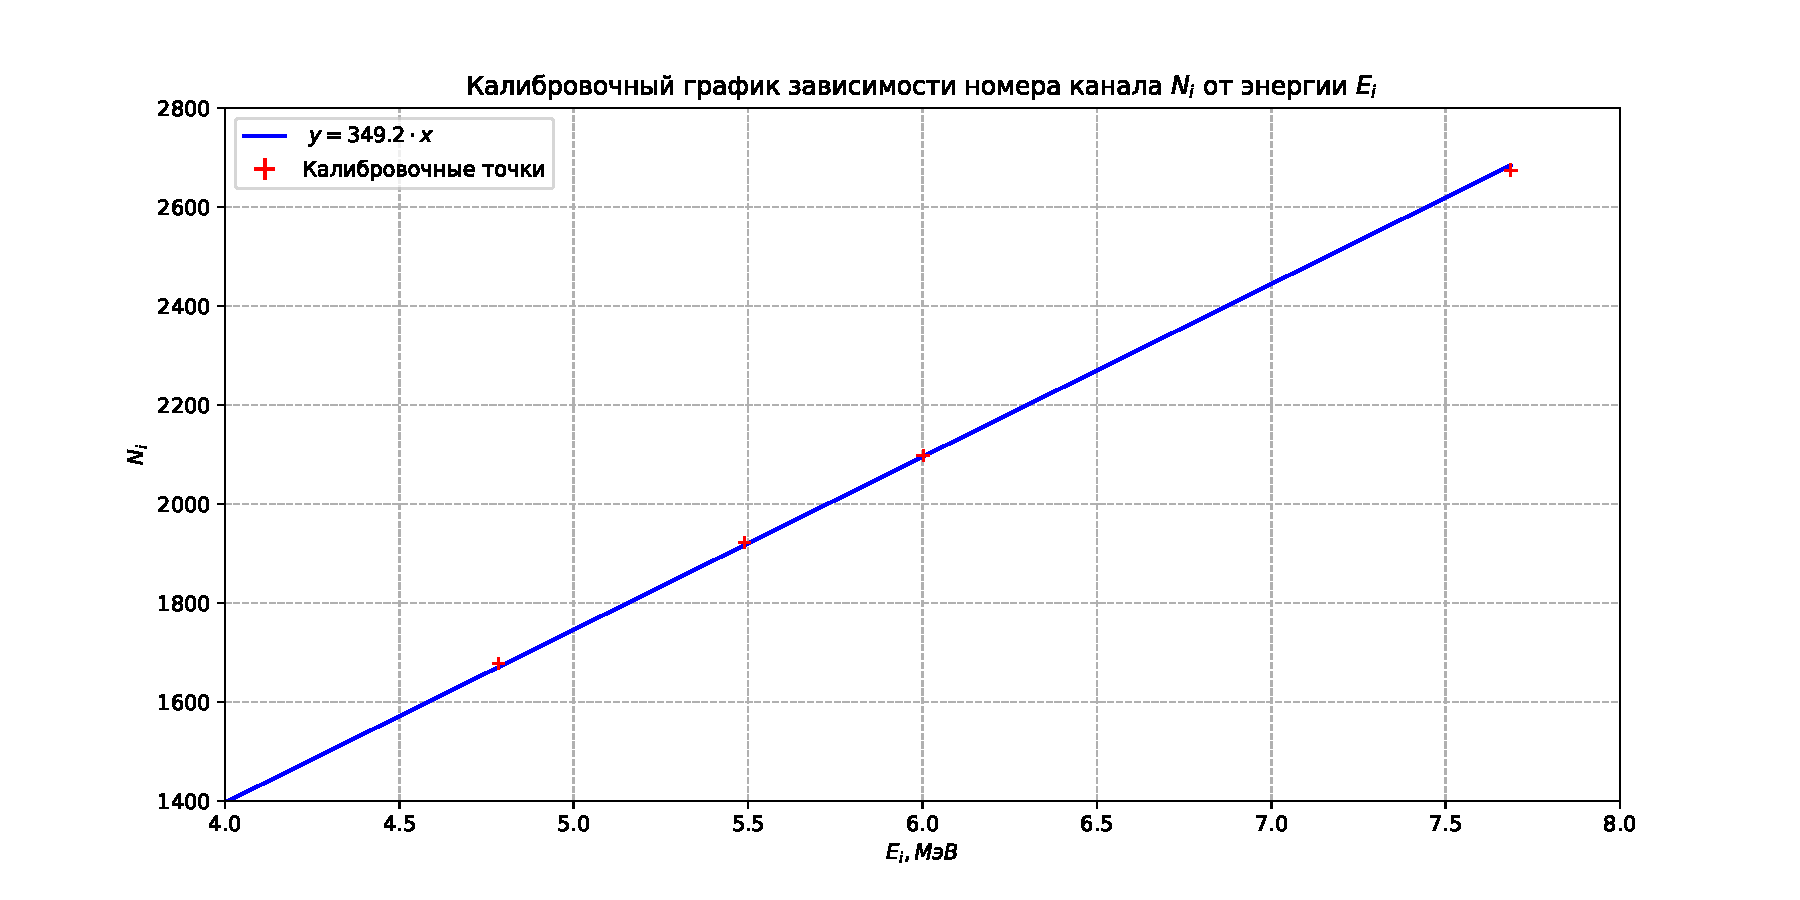
\includegraphics[width=1.1\textwidth]{plots/cal_graph.pdf}
	\caption{\textit{Калибровочный график зависимости $N_i = \alpha E_i$}}
	\label{graph:cal_graph}
\end{figure}
\FloatBarrier

По углу наклона прямой найдем коэффициент $\alpha$ (погрешность вычислим из МНК):

\begin{equation*}
    \alpha = (349.2 \pm 0.6) \ \text{МэВ}^{-1}
\end{equation*}

Прокалибруем все измерения и изобразим спектры на рис. \ref{graph:Ra}, \ref{graph:Am_Th}, \ref{graph:Pu} и \ref{graph:U} и отметим на них положения пиков.




\begin{enumerate}[resume]
    \item Используя калибровочный график, определим для всех остальных пиков значения энергии пиков $E_i$, их ширину $\Delta E_i$ и энергетическое разрешение $R_i = \Delta E_i / E_i$. Результаты запишем в таблицу \ref{table:2}.
\end{enumerate}

\begin{table}[!ht]
    \centering
    \begin{tabular}{|l|l|l|l|l|l|l|l|}
        \hline
        источник & $N_i$ & $\Delta N_i$ & $E_i$, МэВ  & $\Delta E_i$, МэВ & $\sigma_E$, МэВ & $R_i$ & $\sigma_{R_i}$  \\ \hline
        Am + Th & 1647.7 & 24.6  & 4.72 & 0.07 & 0.01 & 0.015 & 0.002 \\ \hline
        Am + Th & 1926.8 & 25.8  & 5.52 & 0.07 & 0.01 & 0.013 & 0.002 \\ \hline
        Pu      & 1811.7 & 23.6  & 5.19 & 0.07 & 0.01 & 0.013 & 0.002 \\ \hline
        Pu      & 1927   & 17.2  & 5.52 & 0.05 & 0.01 & 0.009 & 0.002 \\ \hline
        U       & 1435   & 66.5  & 4.11 & 0.19 & 0.01 & 0.046 & 0.003 \\ \hline
        U       & 1621   & 106.6 & 4.64 & 0.31 & 0.01 & 0.066 & 0.005 \\ \hline
    \end{tabular}
    \caption{Вычисление энергий пиков и их энергетического разрешения}
    \label{table:2}
\end{table}


Погрешность $E$ вычислим по формуле:

\begin{equation*}
    \sigma_E = E \sqrt{\left(\frac{\sigma_N}{N}\right)^2 + \left(\frac{\sigma_\alpha}{\alpha}\right)^2}
\end{equation*}

И запишем в таблицу \ref{table:2}. Погрешность $R$ вычислим аналогично и запишем в таблицу \ref{table:2}.


\begin{enumerate}[resume]
    \item Определим энергетическое разрешение при распаде $\prescript{226}{88}{\text{Ra}}$, связанное с флуктуацией числа образующихся электронно-дырочных пар, которые создаются $\alpha$-частицей в детекторе.
\end{enumerate}


\begin{equation}\label{eq:12}
    R_\text{фл} = \frac{1}{\sqrt{N}} = \sqrt{\frac{E}{E_\text{ср}}},
\end{equation}

где $E_\text{ср} = 3.6$ эВ -- средняя энергия создания пары электрон-дырка. Тогда посчитаем разницу энергетического разрешения $\Delta R$, связанную с шумом в электрической цепи детектора:

\begin{equation}
    \Delta R = R_i - R_{\text{фл}, i}
\end{equation}

и запишем в таблицу \ref{table:3}. Погрешность посчитаем через частные производные


\begin{table}[!ht]
    \centering
    \begin{tabular}{|l|l|l|l|l|}
        \hline
        Номер пика & 1   & 2   & 3   & 4   \\ \hline
        $\Delta R \cdot 10^6$          & 867 & 810 & 774 & 684 \\ \hline
        $\sigma_{\Delta R} \cdot 10^6$ & 6   & 6   & 5   & 5   \\ \hline
    \end{tabular}
    \caption{Вычисление энергетического разрешения, связанного с флуктуацией числа электронно-парочных дыр}
    \label{table:3}
\end{table}

Тогда $\Delta R$ вычислим как среднее, а погрешность как стандартное среднеквадратичное отклонение:

\begin{equation*}
    \Delta R = (13 \pm 3) \cdot 10^{-3}
\end{equation*}

\begin{enumerate}[resume]
    \item Проверим выполняется ли закон Гейгера-Неттола. Построим график зависимости $\lg{T_{1/2}}$ от $1 / \sqrt{E_\alpha}$ для $\prescript{226}{88}{\text{Ra}}$.
\end{enumerate}

Запишем периоды полураспада в таблицу \ref{table:4}.

\begin{table}[!ht]
    \centering
    \begin{tabular}{|l|l|l|l|l|}
        \hline
        ~              & 1   & 2   & 3   & 4   \\ \hline
        $T_{1/2}$, с   & $5.1 \cdot 10^{10}$ & $3.3\cdot 10^{5}$ & $1.87\cdot 10^{2}$ & $1.63 \cdot 10^{-4}$ \\ \hline
    \end{tabular}
    \caption{Периоды полураспада для дочерних ядер $\prescript{226}{88}{\text{Ra}}$}
    \label{table:4}
\end{table}


Если закон выполняется, то зависимость имеет вид:
\begin{equation*}
    \lg{T_{1/2}} = \frac{a}{\sqrt{E_\alpha}} + b,
\end{equation*}
где $a \simeq 1.6 Z = 141$ и $b \simeq -1.6 Z^{2/3} - 21.4 = -53$, $Z = 88$. График изобразим на рис. \ref{graph:lgT}, так же изобразим прямую с теоретически предсказанными коэффициентами.

Коэффициенты:

\begin{equation*}
    a = (150 \pm 9), \ \ \ b = (-58 \pm 4)
\end{equation*}

Посчитаем метрику $\chi^2$, чтобы определить, выполняется ли закон:

\begin{equation*}
    \chi^2 = \sum \frac{\left(y - \hat{y}\right)^2}{\sigma_y^2 + \sigma_{\hat{y}}^2}
\end{equation*}

где, $y$ - значения экспериментальных точек, $\hat{y}$ - аппроксимация, $\sigma_y$ и $\sigma_{\hat{y}}$ - погрешности $y$ и $\hat{y}$ соответственно.

\begin{equation*}
    y = \log{T_{1/2}}, \ \ x = \cfrac{1}{\sqrt{E_\alpha}}
\end{equation*}
Погрешности:

$ \sigma_y = \left| \frac{\partial y}{\partial T_{1/2}} \right| \sigma_{T_{1/2}} = \frac{1}{\ln{10}} \varepsilon_{T_{1/2}} $

$ \sigma_z = \left| \frac{\partial x}{\partial E_\alpha} \right| \sigma_{E_\alpha} = \left(  \frac{1}{2} E_\alpha^{-3/2} \right) \sigma_{E_\alpha} = \frac{x}{2} \varepsilon_{E_\alpha}$

Для аппроксимации:
\begin{equation*}
    \hat{y} = ax + b, \ \ \ \sigma_{\hat{y}} = \sqrt{ \left( \cfrac{\partial \hat{y}}{\partial x} \right)^2 \sigma_x^2 + \left( \cfrac{\partial \hat{y}}{\partial a} \right)^2 \sigma_a^2 + \left( \cfrac{\partial \hat{y}}{\partial b} \right)^2 \sigma_b^2 } = \sqrt{ a^2 \sigma_x^2 + x \sigma_a^2 + \sigma_b^2 }
\end{equation*}

Тогда получаем:

\begin{equation*}
    \chi^2 \approx 0.03
\end{equation*}

Так как значение метрики $\chi^2$ ниже 1, то можно утверждать, что закон выполняется с хорошей точностью.


\begin{figure}[!ht]
	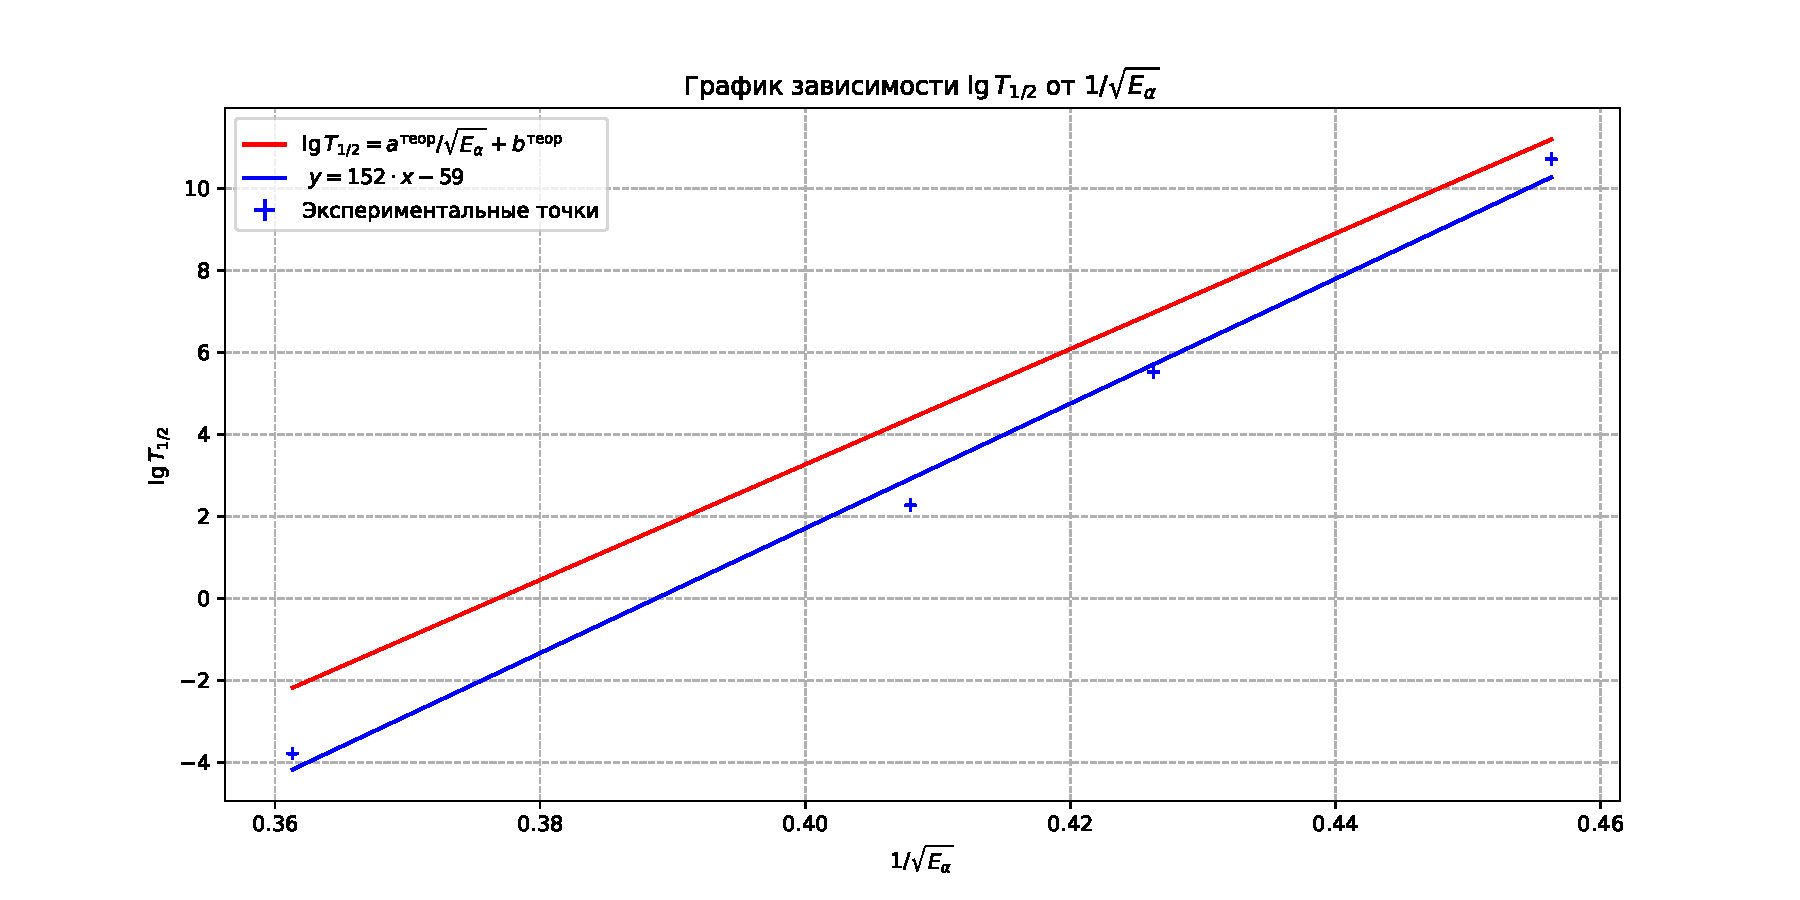
\includegraphics[width=1.1\textwidth]{plots/graph_lgT.pdf}
	\caption{\textit{График зависимости $\lg{T_{1/2}}$ от $1 / \sqrt{E_\alpha}$}}
	\label{graph:lgT}
\end{figure}


\section{Выводы}

\begin{enumerate}
    \item Получены спектры $\alpha$-частиц, испускаемых изотопами: $\prescript{226}{88}{\text{Ra}}, \prescript{241}{95}{\text{Am}} + \prescript{230}{90}{\text{Th}}, \prescript{239}{94}{\text{Pu}}$ и $\text{U}_\text{пр}$.
    \item Была определена энергия $\alpha$-частиц и энергетическое разрешение.
    \item Было проверено, что выполняется закон Гейгера-Неттола.
\end{enumerate}


\FloatBarrier
\begin{figure}[!ht]
	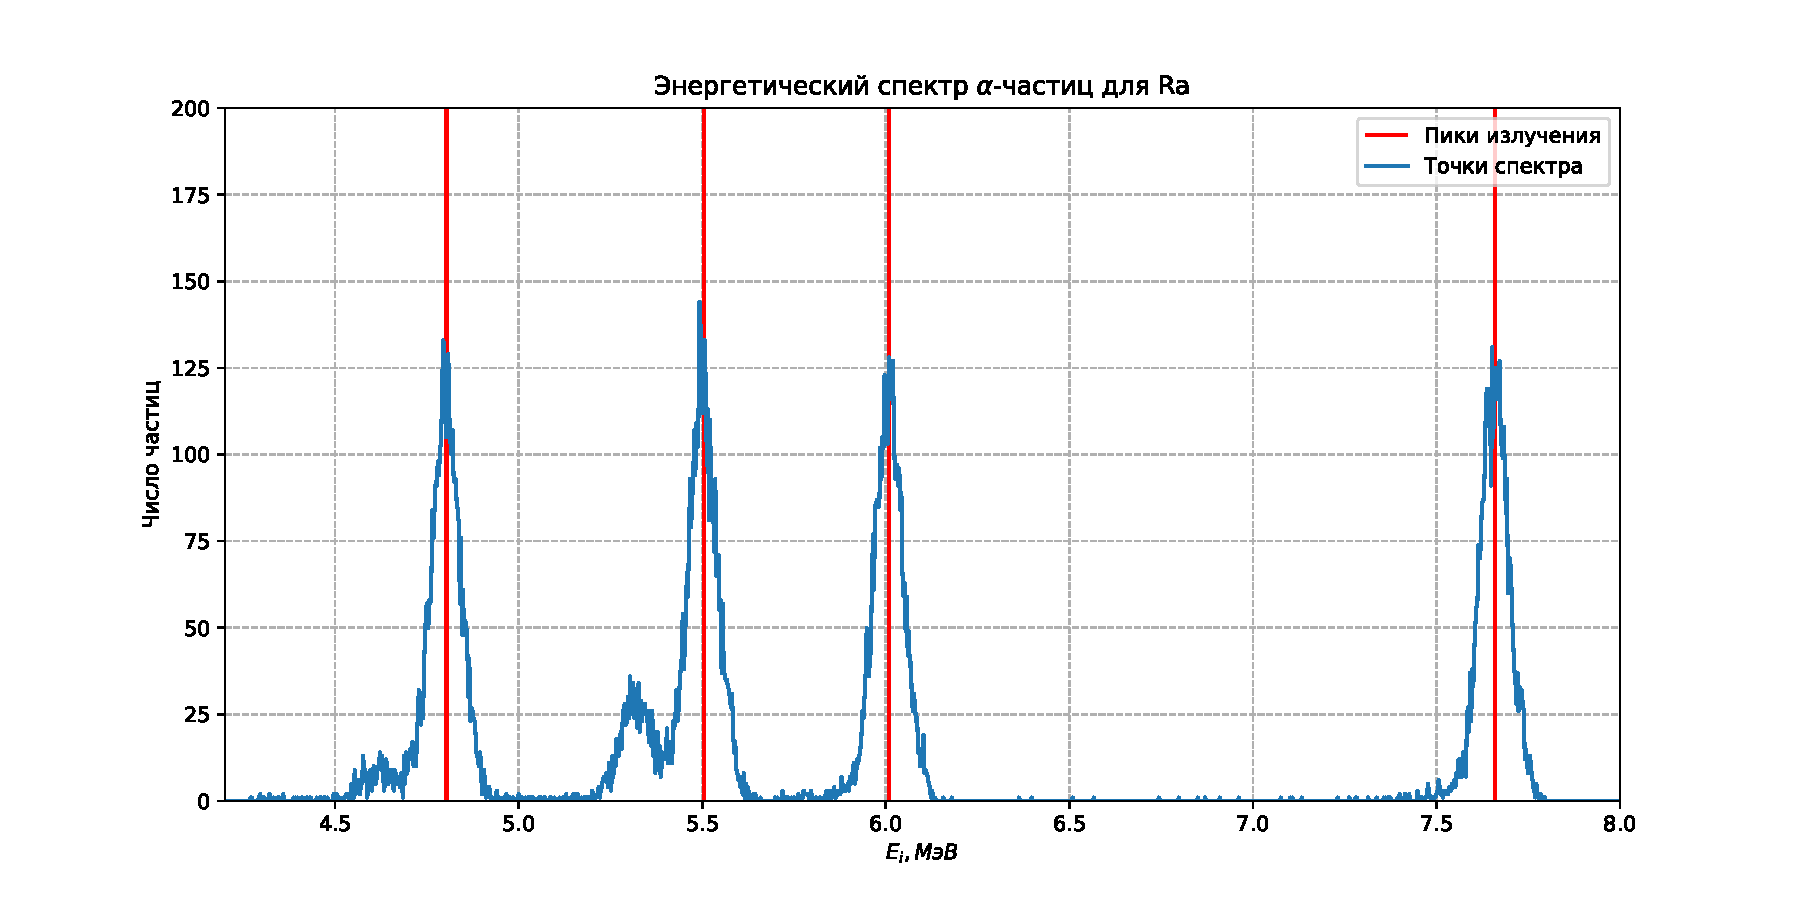
\includegraphics[width=1.1\textwidth]{plots/specter_Ra.pdf}
	\caption{\textit{Спектр $\alpha$-излучения для $\prescript{226}{88}{\text{Ra}}$}}
	\label{graph:Ra}
\end{figure}

\begin{figure}[!ht]
	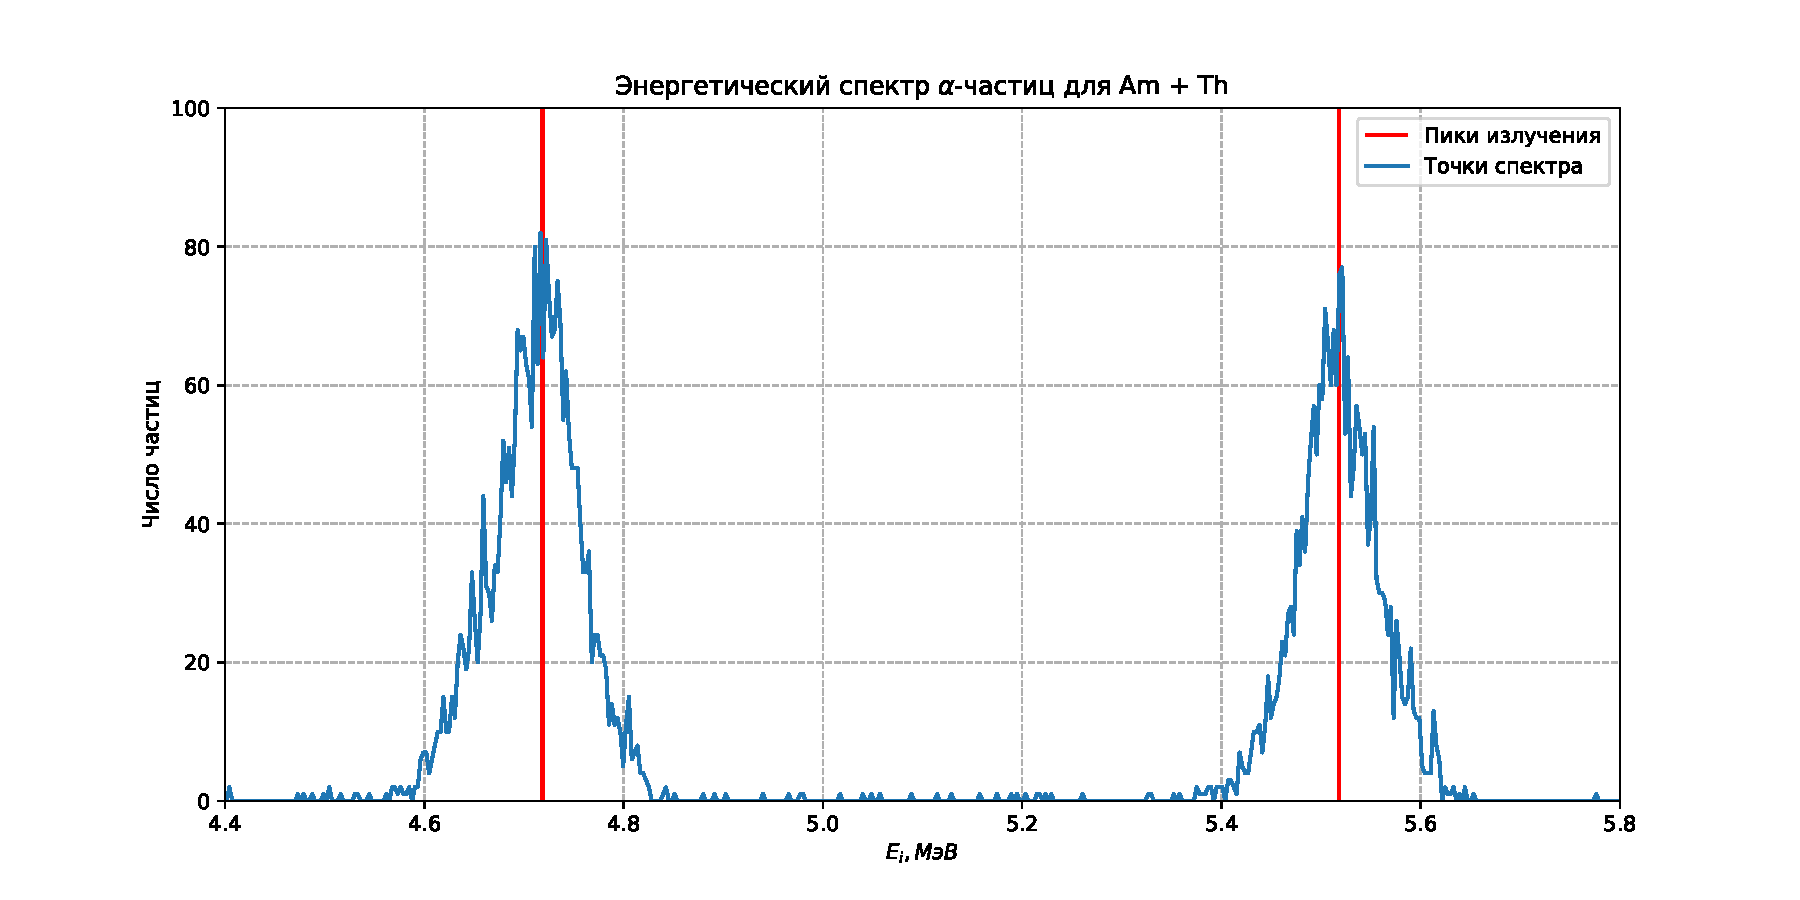
\includegraphics[width=1.1\textwidth]{plots/specter_Am_Th.pdf}
	\caption{\textit{Спектр $\alpha$-излучения для $\prescript{241}{95}{\text{Am}} + \prescript{230}{90}{\text{Th}}$}}
	\label{graph:Am_Th}
\end{figure}

\begin{figure}[!ht]
	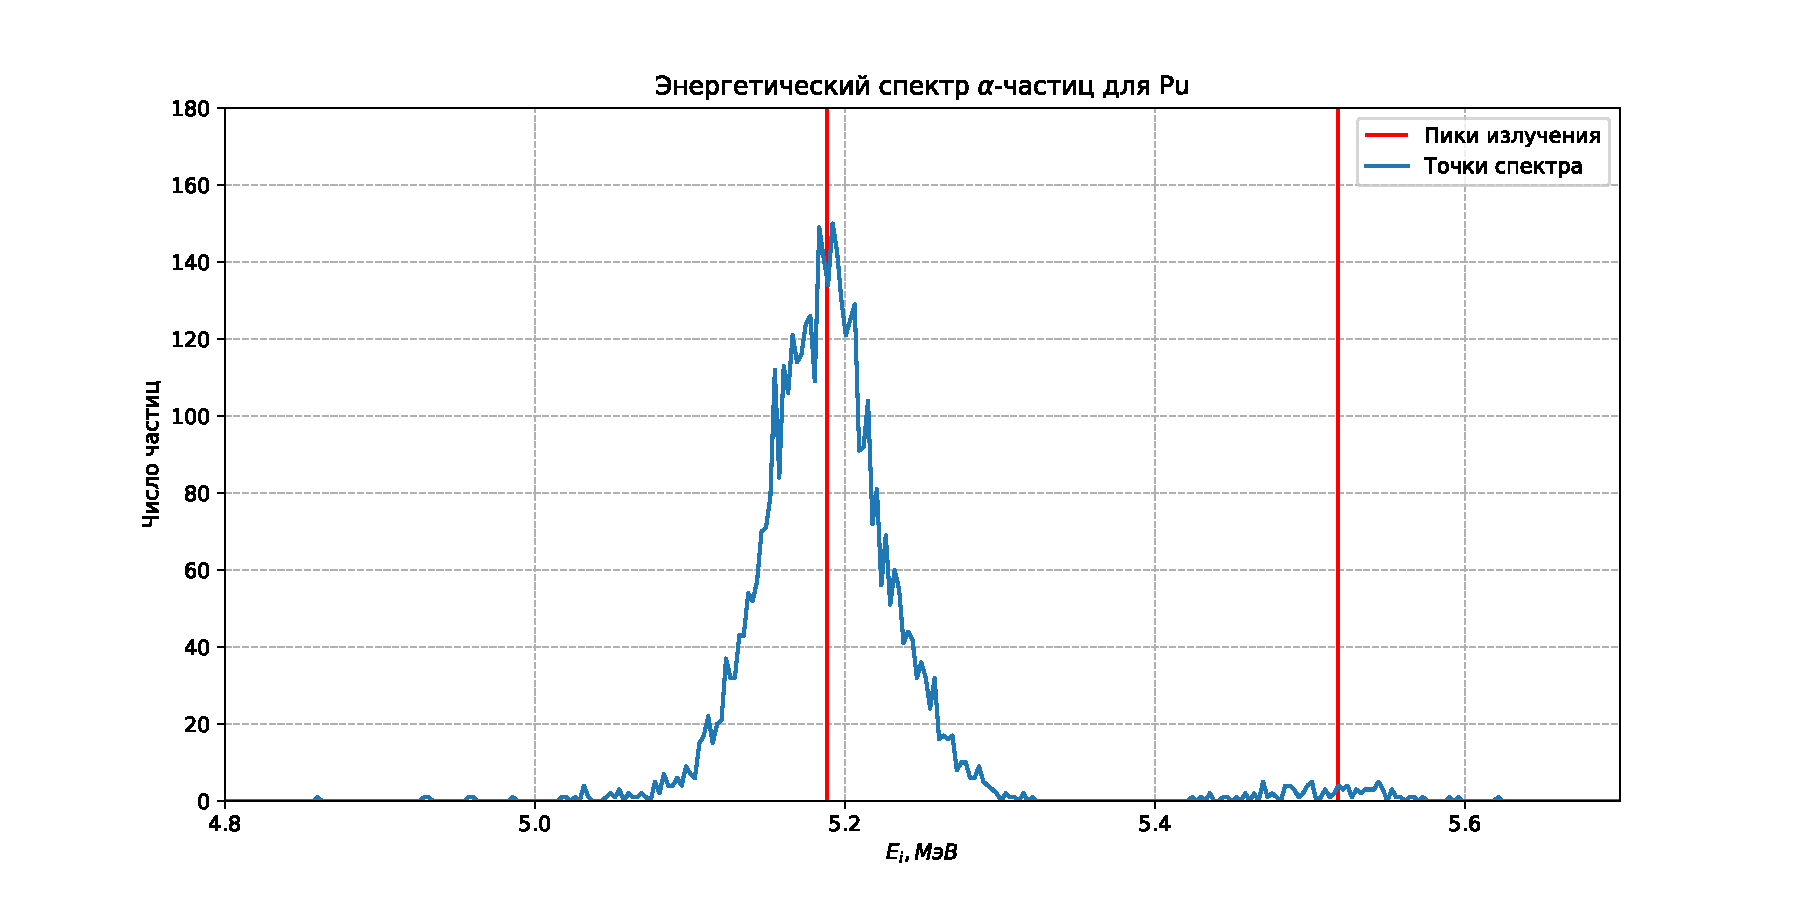
\includegraphics[width=1.1\textwidth]{plots/specter_Pu.pdf}
	\caption{\textit{Спектр $\alpha$-излучения для $\prescript{239}{94}{\text{Pu}}$}}
	\label{graph:Pu}
\end{figure}

\begin{figure}[!ht]
	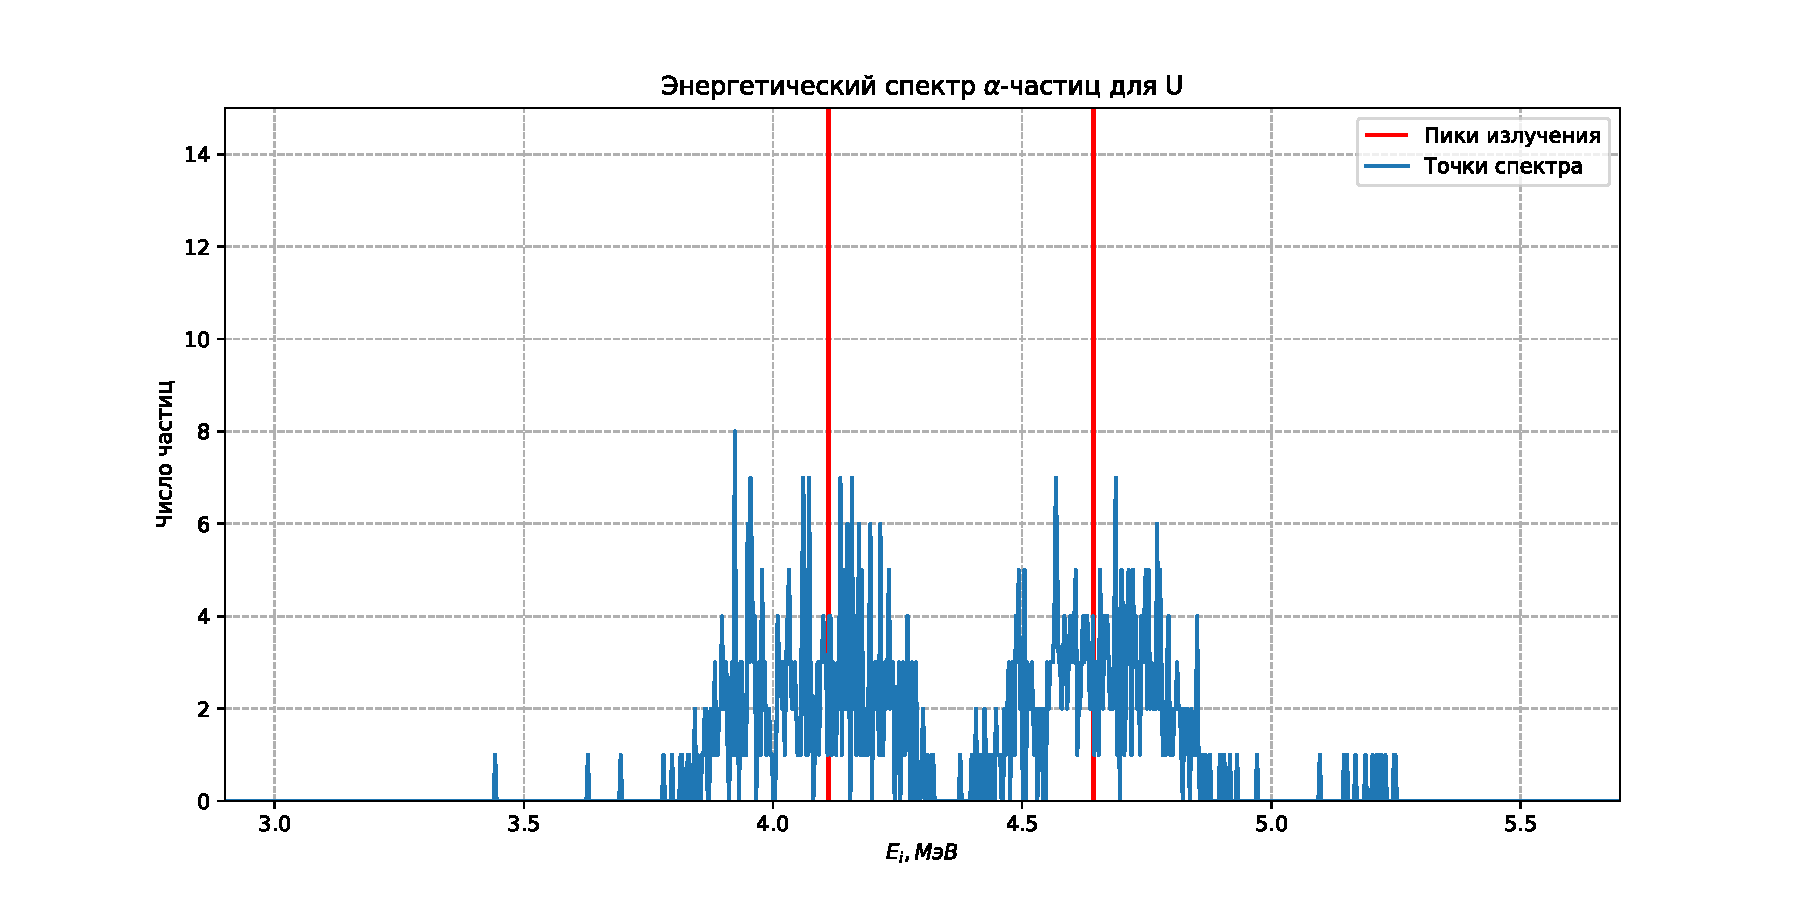
\includegraphics[width=1.1\textwidth]{plots/specter_U.pdf}
	\caption{\textit{Спектр $\alpha$-излучения для $\text{U}_\text{пр}$}}
	\label{graph:U}
\end{figure}
\FloatBarrier


\end{document}
